\section{Motivation}
\label{sec:motivation}

\acrfull{optimization} problems are ubiquitous in real-world scenarios. Consider, for
example, the task planning a road trip, which involves various optimization
challenges. These range from selecting the best route considering factors like
fuel efficiency, travel time, and budget limitations, to efficiently packing
luggage. Solving these problems entails finding good feasible solutions, ideally
in most time-efficient manner possible.

Tackling an optimization problem typically begins by understanding the problem
and its details. Then, a strategy is employed to solve the problem. This
highlights the two main steps: first, describing the problem's details to
construct a representation (model), and second, using the gathered information
to employ a strategy (solver) aimed at discovering feasible solutions.

In fact, this approach serves as the foundation for one of the most widely
employed methods used to address optimization problems, wherein a standard
mathematical formulation (model) describing the problem is developed.
Subsequently, one of the numerous available generic solvers, such as the
``simplex'' algorithm, is utilized to find solutions. Notably, ``simplex'',
being an exact solver, ensures the optimality of the obtained solutions.

Although this method for solving optimization problems is clearly established in
the community there is recently growing interest in how to employ heuristic and
meta-heuristic strategies to solve these problems, specifically, in the
~\acrfull{combinatorial-optimization} field.

\acrfull{heuristic} methods are a set of, often problem-specific, procedures
that attempt to quickly solve a problem and provide a helpful ``rule of thumb''
for achieving reasonably good results, usually in a greedy fashion.~\acrfull{meta-heuristic} methods combine several subordinate heuristics thus
being more generic and can be applied to broad a range of problems. Natural
processes and phenomena, such as collective behavior, natural selection, and
some physical properties of materials, inspire several meta-heuristic search
processes making them flexible and adaptable, although more computationally
intensive than more conventional heuristics. Remarkably, both strategies are
generally more time-efficient than exact approaches, though without an
associated guarantee of optimality.

Given the nature of~\acrlong{heuristic} and~\acrlong{meta-heuristic} methods, and the inherent
diversity of problems, crafting universal meta-heuristic solvers is challenging.
Unlike mathematical optimization, there's no established modelling framework for
meta-heuristics that follows the same principled approach, possibly due to
skepticism about its feasibility and effectiveness.

The establishment of this framework would standardize problem-solving
approaches, facilitate the reuse of meta-heuristic methods, and distinctly
separate the tasks of problem modeling and solver development. Moreover, it
would provide researchers and practitioners with a useful tool to experimentally
assess the performance of~\acrlong{meta-heuristic} methods across a range of diverse
problems.

\begin{figure}[h]
  \centering
  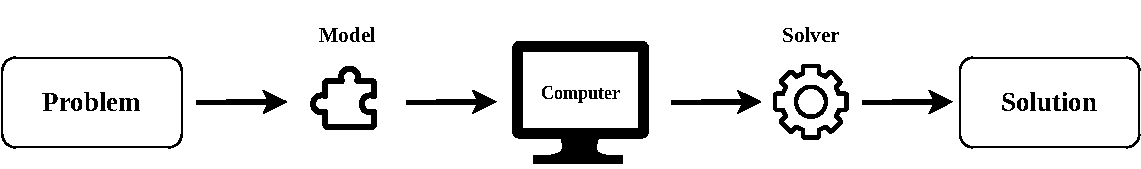
\includegraphics[width=\textwidth,keepaspectratio]{../assets/modelling/modelling.pdf}
  \caption{Modelling and Problem Solving}
  \label{fig:problem-solving}
\end{figure}

In summary, the concept of a modeling framework for problem tackling can be
visually depicted as shown in \Vref{fig:problem-solving}. For a given
problem, a computational model that describes the problem is generated and
provided to a machine, which then employs a meta-heuristic solver to acquire
solutions. This approach is built upon prior
work~\cite{vieira2009uma,outeiro2021application} that has initiated the
formalization of this objective.

Simultaneously, alongside the development and application of meta-heuristic
strategies to address combinatorial optimization problems, there exists a
community interest in constructing a collection of benchmark optimization
problems that hold both theoretical and practical significance. The Google Hash
Code Competition problems, arguably, present themselves as suitable candidates.

The Hash Code programming competition, formerly hosted annually by Google,
challenged teams of up to four members to solve intricate problems within a
four-hour time frame. Participants were allowed to use any tools, resources, and
programming languages of their choice. These problems often drew inspiration
from real-world issues and engineering challenges, such as vehicle routing, task
scheduling, and Wi-Fi router placement. Essentially, can be classified as
``open'' research problems. Importantly, if not entirely, the majority of these
problems can be classified as \acrlong{combinatorial-optimization} problems.

Given the pertinence of these problems, they serve as apt benchmarks for the
evaluation of meta-heuristics. Moreover, they offer a suitable approach to
assess the feasibility of the aforementioned principled modeling approach. Not
only do these problems present challenges from theoretical and practical
standpoints, but they are also have well written and detailed statements. The
competition context in which they were presented also provides a wealth of
empirical data regarding the best solutions attained thus far.